\documentclass[crop,tikz]{standalone}
\usetikzlibrary{%
    arrows,
    arrows.meta,
    automata,
    backgrounds,
    calc,
    decorations.pathreplacing,
    fit,
    matrix,
    positioning,
    scopes,
    shadows
}
\usepackage[linguistics]{forest}
\usepackage[charter]{mathdesign}
\tikzset{headarrow/.style = {-{Latex[length=.5em]}}}

\begin{document}
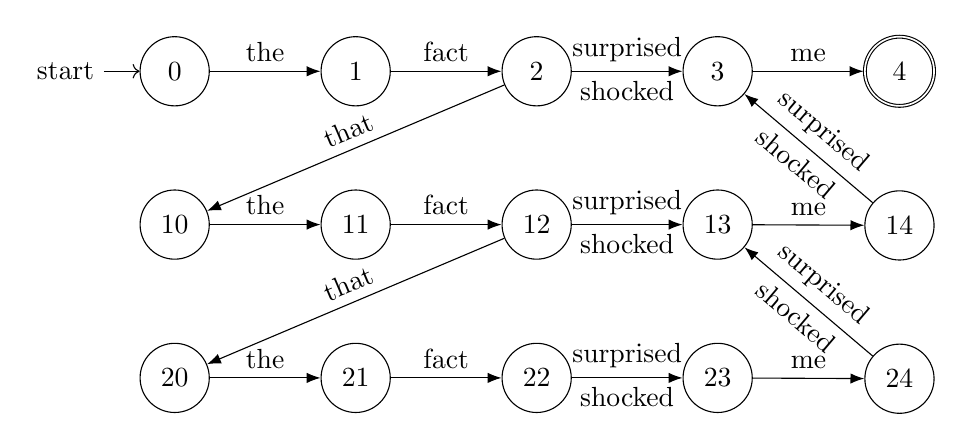
\begin{tikzpicture}
    \node[state,initial] (0-0) at (0,0) {0};
    \foreach \x [remember=\x as \lastx (initially 0)] in {1,2,3}
        \node[state] (0-\x) [right=4em of 0-\lastx] {\x};
    \node[state,accepting] (0-4) [right=4em of 0-3] {4};

    \foreach \x in {0,...,4}
        {
        \node[state] (1-\x) [below=3em of 0-\x] {1\x};
        \node[state] (2-\x) [below=3em of 1-\x] {2\x};
        }

    \foreach \x/\Label [remember=\x as \lastx (initially 0)] in {%
        1/the,
        2/fact,
        3/surprised,
        4/me%
        }
        {
        \draw[headarrow] (0-\lastx) to node [above] {\Label} (0-\x);
        \draw[headarrow] (1-\lastx) to node [above] {\Label} (1-\x);
        \draw[headarrow] (2-\lastx) to node [above] {\Label} (2-\x);
        }

    \draw[headarrow] (0-2) to node [above,sloped] {that} (1-0);
    \draw[headarrow] (1-2) to node [above,sloped] {that} (2-0);
    \draw[headarrow] (1-4) to node [above,sloped] {surprised} (0-3);
    \draw[headarrow] (2-4) to node [above,sloped] {surprised} (1-3);

    \foreach \x in {0,1,2}
        \path (\x-2) to node [below] {shocked} (\x-3);
    \path (1-4) to node [below,sloped] {shocked} (0-3);
    \path (2-4) to node [below,sloped] {shocked} (1-3);
\end{tikzpicture}
\end{document}
